\section{Approaches}

This section discusses the optimization of the two enumerators from the previous section, each using a different approach. In addition, a third approach discussed is to avoid scanning unsupported services. 

\subsection{Use information of a former service scan}

This approach aims to reuse information from one enumerator in a later enumerator within the same scan. This will be applied to the RCEnumerator.

\subsubsection{Current behavior}

The Routine Control service is used by the client to execute a defined sequence of steps and obtain any relevant results \cite{iso14229}. For a quick overview of the service a simplified code snippet of the Scapy implementation is used.

\begin{samepage}
\begin{minted}{python}
class UDS_RC(Packet):
    routineControlTypes = {
        1: 'startRoutine',
        2: 'stopRoutine',
        3: 'requestResults'
    }
    fields_desc = [
        ByteEnumField('routineControlType', 0, routineControlTypes),
        XShortField('routineIdentifier', 0)
    ]
\end{minted}
\end{samepage}

The \mintinline{python}{routineControlType} field specifies what should happen to a routine. Possible are starting, stopping and requesting the results. To specify which routine is to be controlled, there is the \mintinline{python}{routineIdentifier} field. Hence, there are three control types, and because the identifier is a short field, there are 2\textsuperscript{16} identifiers. This leads to the following formula, showing how many requests are generated for a UDS scan:
\[f(n)=3 \cdot 2^{16} \cdot n\]
wherin $n$ stands for the number of detected states.

The current RCEnumerator does exactly this, it generates the full range for each state. That's what needs to be reduced. Its current behavior is illustrated in \autoref{fig:rc-behavior-current}. The green areas symbolize the scanned ranges.

\begin{figure}[h]
    \centering
    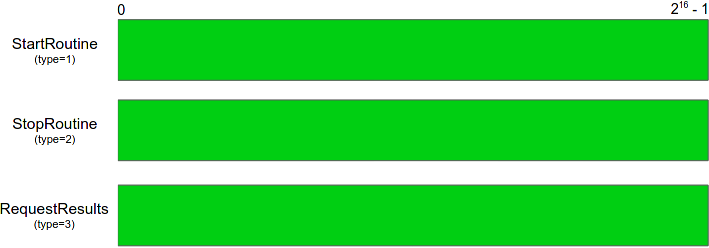
\includegraphics[width=0.8\textwidth]{rc-behavior-current}
    \caption{Current procedure for scanning the RC service.}
    \label{fig:rc-behavior-current}
\end{figure}

\subsubsection{Elaborating the new behavior}

As a first step to find a way to apply the approach to the RCEnumerator, the distribution of the identifiers is visualized grouped by the type as a histogram in \autoref{fig:rc-distribution}.

% TODO: maybe to attachments
\begin{figure}[h]
    \centering
    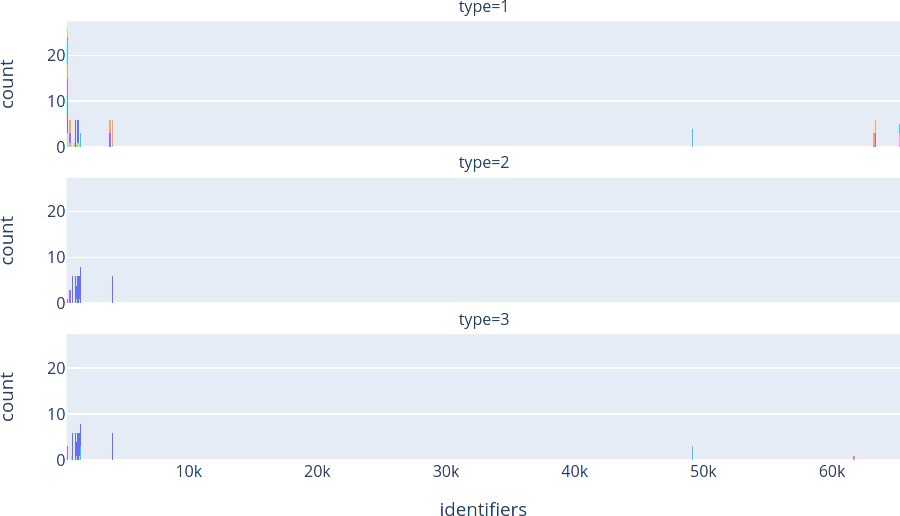
\includegraphics[width=0.8\textwidth]{rc-distribution}
    \caption{Distribution of the RC identifiers. Each color is one ECU.}
    \label{fig:rc-distribution}
\end{figure}

It can be seen that if an identifier is available in Type1, it is likely that this identifier also occurs in Type2. Consequently, if an identifier does not respond positively in Type1, it is also very unlikely that it will respond in Type2 or Type3. This appearance is used to reduce the scan range for this service.

The new behavior starts with scanning all 2\textsuperscript{16} identifiers with Type1. So, 2\textsuperscript{16} is the minimum number of requests for each state with the new behavior. Only the identifiers, which led to a positive response, are scanned with Type2 and Type3 as well. Moreover, it was observed that there seems to be a locality effect for the identifiers. Thus, if an identifier with Type1 is answered positively, scanning nearby identifiers instead of just that identifier will result in higher coverage. What needs to be found out is the block size which leads to the best coverage, while maintaining an appropriate speed-up. \autoref{fig:rc-behavior-new} illustrates that. The green areas again show the scanned ranges, additionally, the red areas are the found identifiers in Type1 and their resulting ranges for Type2 and Type3 and the gray areas show the areas that were not scanned and thus how much time was saved.

\begin{figure}[h]
    \centering
    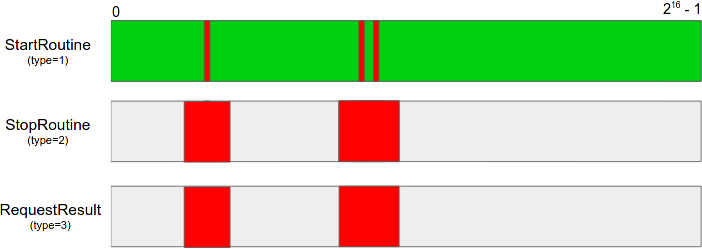
\includegraphics[width=0.8\textwidth]{rc-behavior-new}
    \caption{New procedure for scanning the RC service.}
    \label{fig:rc-behavior-new}
\end{figure}

The limits of the speed-up are defined as following:
\[ 0\ \% \ \leq\  s(n)\  \leq 66.\overline{6}\ \% \quad \forall \  n \in \left\{0, 1, ..., 2^{16} \cdot 3\right\} \]
%\[ 0\  \ \leq\  s(n)\  \leq \frac{2}{3} \quad \forall \  n \in \left\{0, 1, ..., 2^{16 * 3}\right\} \]
wherin $s$ is the speed-up function and $n$ the number of generated requests for this service.

The reason for the upper limit of $66.\overline{6}$ \% is that Type1, which is one third of all possible requests, is always scanned completely.

To find out the best value, scans with different block sizes are simulated. For a quick simulation another observation is used. If one identifier is available in one state, it is likely to be available in the other states too. Thus, the states are ignored in the simulation, which improves the performance by a multiple, while it is still very close to the real ECUs. The simulation only uses information gathered from the real ECUs as described in \autoref{sec:data-gathering}. Specifically, the required information is extracted from the generic.log file.

As described, the simulation starts with getting all identifiers which have been positively answered by the currently simulated ECU. Subsequently, these identifiers are expanded to both sites from 0 to 200. Overlapping blocks are resolved to one continuous space. With these blocks the coverage and the number of requests can be calculated. The number of requests can be converted to the speed-up. The results are averaged.
The blocks are expanded to both sites. So, for example, if the identifier 500 has been answered positively and the expansion size is 100, it leads to block from 400 to 600. A simulation was also run with expanding individual identifiers in to one site only, which yielded very similar results. Thus, it was left with the expansion in both directions. 
The following pseudocode shows the procedure more clearly.

\begin{samepage}
\begin{minted}{python}
coverages = []
speedups = []
for expansion_size in range(200):
    coverages_block = []
    speedups_block = []
    for ecu in ecus:
        ids_type1 = get_type1_ids(ecu)
        to_scan = ids_to_block(ids_type1, expansion_size)
        coverages_block.append(get_coverage(ecu, to_scan))
        count_requests = len(to_scan)
        speedups_block.append(get_speedup(ecu, count_requests))
    coverages.append(avg(coverages_block))
    speedups.append(avg(speedups_block))
\end{minted}
\end{samepage}

The results of this simulation are plotted in \autoref{fig:rc-simulation-result}. The speed-up is linear to the expansion size. That makes sense, because the larger the blocks are, the more requests are generated. The expansion size of zero represents the results without using the locality effect. The maximum difference in coverage between with and without locality effect are 22\%, even though the maximum speed-up difference is only 1\%.

\begin{figure}[h]
    \centering
    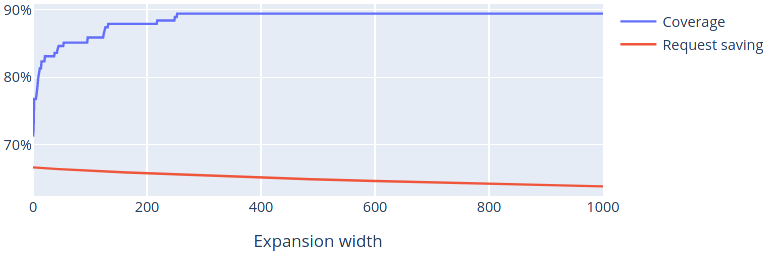
\includegraphics[width=0.7\textwidth]{rc-simulation-result}
    \caption{Simulation result for the RC enumerator.}
    \label{fig:rc-simulation-result}
\end{figure}

Since the speed-up is high for each simulated block size, the highest coverage was chosen which starts with block size \textbf{132}. Hence, this value is the chosen and implemented block size.

\subsubsection{Implementation}

Three classes are of interest:

\begin{itemize}
    \item \textbf{RCEnumerator}: Defaults to scanning the whole RC service, including all three types.
    \item \textbf{RCStartEnumerator}: Only scanning Type1 of the RC service.
    \item \textbf{RCSelectiveEnumerator}: Staged enumerator containing an RCStartEnumerator and an RCEnumerator.
\end{itemize}

\begin{figure}[h]
    \centering
    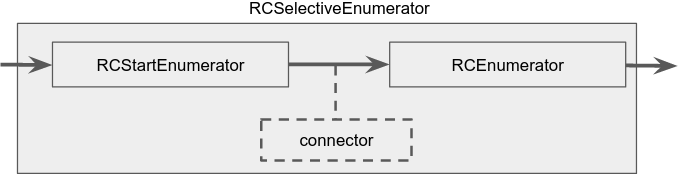
\includegraphics[width=0.7\textwidth]{rc-schematic}
    \caption{Schematic illustration of the new RCSelectiveEnumerator.}
    \label{fig:rc-schematic}
\end{figure}

The RCSelectiveEnumerator connects its two stages with a connector function that is called as soon as the first stage is done and the second is to be started. It expands the found identifiers of the RCStartEnumerator to ranges and also resolves any overlaps to a continuous range and forwards these ranges to the second stage, the RCEnumerator. Additionally, the connector configures the RCEnumerator to only scan Type2 and Type3.

Each positively answered identifier of Type1 in any state will also be probed for all subsequent states in Type2 and Type3, even if this identifier is not found in Type1 for another state. This increases the coverage in cases, where a routine can be started in a state, but its result, or to stop it, may only be requested in another state. It also hardly leads to more requests, which can be seen at the speed-ups in \autoref{fig:rc-schematic}.

\subsubsection{Evaluation}

\begin{table}[h]
    \begin{center}
    \begin{tabular}{ccc}
        \hline
        & \textbf{Coverage} & \textbf{Speed-up} \\
        \hline
        \textbf{audi\_cgw} & 87.6\% & 65.4\% \\
        \textbf{bfft-ecu} & 100\% & 66.2\% \\
        \textbf{bmw-gateway-ecu-bdc} & 100\% & 66.2\% \\
        \textbf{bmw-gateway-ecu-zgw} & 100\% & 64.5\% \\
        \textbf{bmw-gateway-ecu2} & 100\% & 64.6\% \\
        \textbf{bmw-tcu} & 100\% & 66.7\% \\
        \textbf{bosch-ecu} & 100\% & 64.6\% \\
        \textbf{dashboard} & 50.0\% & 66.2\% \\
        \textbf{mercedes-ezs} & 100\% & 65.1\% \\
        \textbf{seppmed} & 100\% & 66.2\% \\
        \textbf{tesla-airbag-ecu} & 100\% & 66.7\% \\
        \hline

    \end{tabular}
    \end{center}
    \caption{Measured coverages and speed-ups on ECUs with approach 1.}
    \label{tab:evaluation-approach1}
\end{table}

9 of 11 ECUs had a full coverage. The coverage for the dashboard ECU notable low. Therefore, a closer look was taken there again. It turned out that the Dashboard only supports two identifiers. The identifier 515 for Type1 and identifier 61,728 for Type3. The former is detected, but the resulting range for Type3 is far from the identifier 61,728. Hence, the loss and a coverage of 50\%.

The speed-up is calculated by comparing the number of requests sent with the selective enumerator and the number of requests that would have been sent with the old enumerator for an entire scan. For each ECU it is close to the theoretical maximum of $66.\overline{6}$ \%, leading to the evaluation that there is a great potential in this approach.

The use of information within the same scan is applicable to scans of services with multiple fields, as it is the case with the RC service that has the \mintinline{text}{routineControlType} and \mintinline{text}{routineIdentifier} fields. This results in a high scan time for this service and thus a high potential time savings. However, if an identifier is not recognized in the first scan, it will not be recognized in the next scans as well.


\subsection{Reduction of scan range}
Most services are simpler and don't have a type as the RC service but only an identifier. So, reusing information within the same scan is limited. Here the second approach will be applied to the Read Data By Identifier (RDBI) enumerator. The idea is to scan more heavily the blocks where positive behavior is more likely than others. The approach will be applied.

\subsubsection{Current behavior}

The Read Data By Identifier service allows the client to request data record values from the server identified by one or more dataIdentifiers \cite{iso14229}. Again, for a quick overview of the service a simplified code snippet of the Scapy implementation is used.

\begin{samepage}
\begin{minted}{python}
class UDS_RDBI(Packet):
    fields_desc = [
        XShortField('identifier', 0)
    ]
\end{minted}
\end{samepage}

To specify which data record to retrieve, there is the \mintinline{python}{identifier} field. Hence, because the identifier is a short field, there are 2\textsuperscript{16} identifiers. This leads to the following formula, showing how many requests are generated for a UDS scan:
\[f(n)=2^{16} \cdot n\]
wherin $n$ stands for the number of detected states. 

So, the current RDBIEnumerator is very simple. It generates 2\textsuperscript{16} packets counting up from 0 to 65535 and generating for each number a packet with this number as identifier for each state.

\subsubsection{Elaborating the new behavior}

As a first step, the distribution of identifiers over all ECUs is visualized in a histogram to check if there is potential. The result can be seen in \autoref{fig:rdbi-distribution}.

\begin{figure}[h]
    \centering
    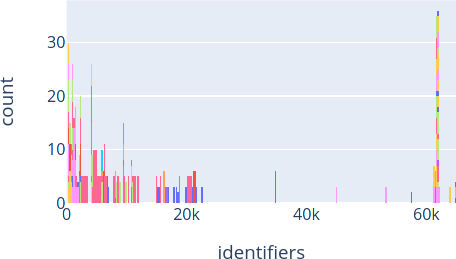
\includegraphics[width=0.7\textwidth]{rdbi-distribution}
    \caption{Distribution of the RDBI identifiers. Each color is one ECU.}
    \label{fig:rdbi-distribution}
\end{figure}

It is clearly visible that there are some areas where not a single identifier was answered positively, and some areas that are particularly covered, such as the beginning and the end. This behavior will be exploited in the remainder of this section.

To reduce this range, first the 2\textsuperscript{16} area is divided into blocks. Then, it is calculated how likely a positive response is for each of these blocks. Based on this information, the number of requests for each block will be calculated individually.
For that, the probability is multiplied with the block size.
\[c(p, s)=\max(p \cdot s, 1)\]
wherin p stands for the probability of the requested block and s for the block size. For each block should be generated at least one request. The requested identifiers within one block are generated randomly. If any of these requests is answered positively in a block, the whole block will be scanned. An example is illustrated in \autoref{fig:rdbi-behavior-new}.

\begin{figure}[h]
    \centering
    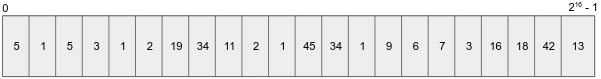
\includegraphics[width=0.7\textwidth]{rdbi-behavior-new}
    \caption{New procedure for scanning the RDBI service.}
    \label{fig:rdbi-behavior-new}
\end{figure}

This leads to one question. Which block size leads to best results? This is again answered by a simulation, which is performed for every possible block size, as such block sizes of $2^2, 2^3, ..., 2^{15}, 2^{16}$ were chosen because they are divisors for 2\textsuperscript{16}. The probability of a positive response of a block are calculated based on the results of all ECUs. The resulting coverage and speed-up are then calculated for each ECU specifically and averaged. The approach has one more feature which makes the simulation more complex than the former simulation. Since the blocks are first scanned randomly, the scan can lead to a great coverage, but also a low one, depending on the hit rate of the generated identifiers. To reduce this effect, the calculation of the coverage and speed-up are made 100 times, each time with newly created random identifiers. The 100 results are averaged to the value corrected from the random factor. This leads to a high processing time. To reduce the runtime, the execution was parallelized.
The following pseudocode shows the procedure more clearly.

\begin{samepage}
\begin{minted}{python}
for exponent in range(2, 16):
    block_size = 2 ** exponent
    coverages = []
    samples = []
    probabilities = get_probabilities(ecus, block_size)
    for ecu in ecus:
        for i in range(100):
            samples = random_samples(block_size, probabilities)
            positive_identifiers = ecu.get_positive_identifiers(samples)
            block_list = to_blocks(positive_identifiers, block_size)
            positive_identifiers = ecu.get_positive_identifiers(block_list)

            coverages.append(get_coverage(ecu, positive_identifiers))
            samples.append(len(block_list))
        avg_coverages, avg_samples = avg(coverages, samples)
\end{minted}
\end{samepage}

This simulation leads to \autoref{fig:rdbi-simulation-result}.

\begin{figure}[h]
    \centering
    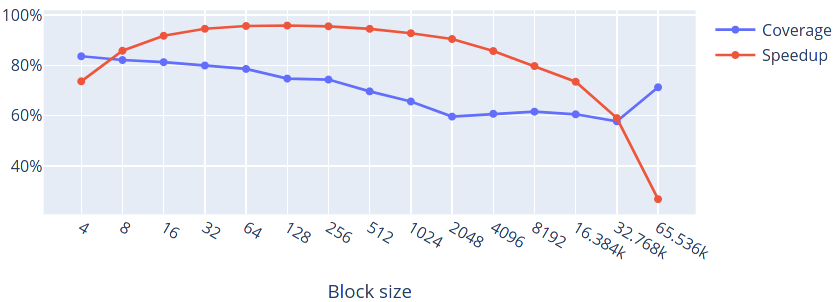
\includegraphics[width=0.8\textwidth]{rdbi-simulation-result}
    \caption{Simulation result for the RDBI service.}
    \label{fig:rdbi-simulation-result}
\end{figure}

The speed-up is no longer linear; instead, the speed-up is highest for medium block sizes. From block sizes 64 to 128, the coverage decreases by 4\% while the speed-up remains the same. Thus, it was decided for \textbf{64} as the block size leading to best results.

\subsubsection{Implementation}

Three classes are of interest again:

\begin{itemize}
    \item \textbf{RDBIEnumerator}: Defaults to scanning the whole RDBI service.
    \item \textbf{RDBIRandomEnumerator}: Scanning block-based with random identifiers.
    \item \textbf{RDBISelectiveEnumerator}: Staged enumerator containing an RDBIRandomEnumerator and an RDBIEnumerator.
\end{itemize}

\begin{figure}[h]
    \centering
    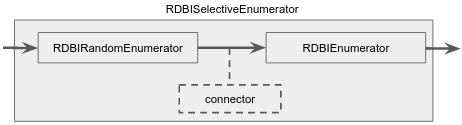
\includegraphics[width=0.7\textwidth]{rdbi-schematic}
    \caption{Schematic illustration of the new RDBISelectiveEnumerator.}
    \label{fig:rdbi-schematic}
\end{figure}

Similar to the previous approach, the new implementation is two-staged. First, the RDBIRandomEnumerator is executed. The connector creates requests for whole blocks, if any identifier of them answered positively. These requests are passed to the configurable RDBIEnumerator. Of course, it is ensured that for a single block each identifier is generated only once.

Also, as with the RCSelectiveEnumerator, each positively answered identifier will be remembered for all subsequent states. This increases the coverage because most identifiers are also available in other states, but the RandomEnumerator might not detect them for each state.

Implementing the RDBIRandomEnumerator was a challenge because it must include the probabilities of occurence of positively responded identifiers for each block. With a block size of $2^6$, there would need to be a list with $\frac{2^{16}}{2^6} = 1024$ elements. Thus, it is desirable to represent this information more compactly. A better representation is based on two facts. That the probabilities are ultimately calculated to the number of samples, and that at least one request shall be generated for each block. For the former, instead of probabilities, the number of samples for each block were pre-computed instead of being computed at runtime. This simplifies the list in the sense that integers are stored instead of float values. Second, the number of samples is not stored for all blocks, but only for blocks whose number of samples is greater than or equal to 2. And blocks for which no value is stored, the value 1 is used. This automatically solves that each block is probed with at least one packet, even if its probability is 0\%. These simplifications transformed the list of 1024 elements into a dictionary of only 109 elements.

\subsubsection{Evaluation}

\begin{table}[h]
    \begin{center}
    \begin{tabular}{ccc}
        \hline
        & \textbf{Coverage} & \textbf{Speed-up} \\
        \hline
        \textbf{audi\_cgw} & 87.8\% & 85.0\% \\
        \textbf{bfft-ecu} & 88.4\% & 96.6\% \\
        \textbf{bmw-gateway-ecu-bdc} & 100\% & 96.1\% \\
        \textbf{bmw-gateway-ecu-zgw} & 94.3\% & 95.8\% \\
        \textbf{bmw-gateway-ecu2} & 83.3\% & 96.1\% \\
        \textbf{bmw-tcu} & 72.2\% & 96.3\% \\
        \textbf{bosch-ecu} & 90.7\% & 93.3\% \\
        \textbf{dashboard} & 92.4\% & 94.4\% \\
        \textbf{mercedes-ezs} & 89.3\% & 94.7\% \\
        \textbf{seppmed} & 83.0\% & 95.9\% \\
        \textbf{tesla-airbag-ecu} & 100\% & 96.4\% \\
        \hline
    \end{tabular}
    \end{center}
    \caption{Measured coverages and speed-ups on ECUs with approach 2.}
    \label{tab:evaluation-approach2}
\end{table}

Overall, the coverages are lower with this approach as for approach 1. Only for two ECUs a coverage of 100\% is reached. It should be noted, that it varies slightly for each run because a random scan is used. The speed-ups are consistently high at approximately 95\%. Nevertheless, the speed-ups of approach 1 are higher in practice, because that approach can be applied to larger service scans, and then a speed-up of about 66\% saves more time there than a speed-up of 95\% here.

The biggest problem with reducing the scan range is the newly added random factor. The coverage can be great for one scan, but low for the next one. This would require performing multiple scans using the new implementation to ensure that most identifiers were found.


\subsection{Avoid the scan of unsupported services}

Each ECU usually supports only a subset of the services offered  by the UDS standard. This approach aims to avoid scanning them in order to save requests and therefore, time.

\subsubsection{Detecting unsupported services}

The first thing to understand is how to tell if a service is supported or not. Figure 5 of the UDS standard shows the general server response behavior. In this work, it can be found in \autoref{fig:server-response-behaviour} and the important area has been highlighted.

\begin{figure}[h]
    \centering
    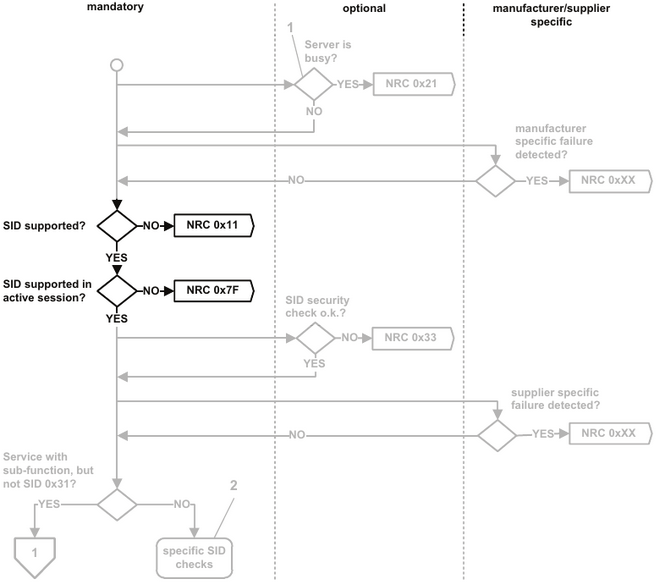
\includegraphics[width=0.8\textwidth]{server-response-behaviour}
    \caption{General server response behavior \cite{iso14229}. SID = service identifier.}
    \label{fig:server-response-behaviour}
\end{figure}

Each request is answered by a response, either positive or negative. A negative response contains a negative response code (NRC). \autoref{fig:server-response-behaviour} shows that 0x11 and 0x7f are relevant for this approach. 0x11 indicates that the requested service is not supported at all. 0x7f is a lighter response code because it shows that the requested service is not supported in the current state of the ECU. Both response codes are sufficient to stop the current enumerator with the current state and start with the next one. Although a 0x11 NRC is received, this service is still probed in other states. This is because with this behavior, in the worst case, one request is generated for this service for each state, which in turn receives 0x11 NRC again and then stops the enumerator. The number of states detected is usually one-digit, so the number of packets generated is negligible. But in the best case the vendor has implemented the NRC incorrectly and the service is available in a different state.

\subsubsection{Implementation}

In contrast to the previous approaches, this one is not applied to an enumerator, but to the UDS Scanner itself. The UDS Scanner evaluates each response, for example to detect if a new state was found. Here, a check was added for negative responses if they have the NRC 0x11 or 0x7f. If they do, the enumerator is set to completed for the currently executed state. This behavior has to be enabled explicitly, because as the next section explains, it might result in losses.

\subsubsection{Evaluation}

\autoref{fig:serviceNotSupported-savings} illustrates the number of saved packets for each ECU with this approach. It is only an approximation because for this graph, the responses with the both described NRCs have been counted. Of course, not every response can be saved with these NRCs, since at least one request must first be made to see the NRC of that service for a state. But this number of requests, as described in the previous paragraph, is very small and negligible, especially considering that the minimum value of saved requests is about 70,000.

\begin{figure}[h]
    \centering
    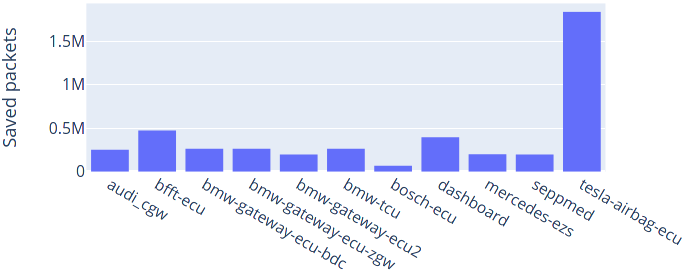
\includegraphics[width=0.8\textwidth]{serviceNotSupported-savings}
    \caption{Saved number of requests with this approach (approx).}
    \label{fig:serviceNotSupported-savings}
\end{figure}

There is one last potential problem with this approach. Reliance is placed on the manufacturer to properly implement these NRCs. It is conceivable that the ECU responds to an identifier with 0x11 or 0x7f, although a subsequent identifier would actually have been answered positively. The occurrences of this behavior are shown in \autoref{fig:serviceNotSupported-losses}. It was calculated by evaluating the responses for each enumerator for each state. Once a negative response with NRC 0x11 or 0x7f was received, an internal counter was incremented with each subsequent positive response.
And in comparison to the potential savings (\autoref{fig:serviceNotSupported-savings}), the losses are negligible.

\begin{figure}[h]
    \centering
    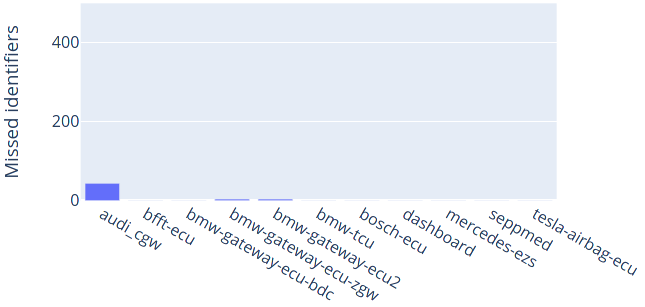
\includegraphics[width=0.8\textwidth]{serviceNotSupported-losses}
    \caption{Lost number of positive responses with this approach.}
    \label{fig:serviceNotSupported-losses}
\end{figure}

Avoiding scanning unsupported services is the safest way to save time of all three approaches. It is unlikely that identifiers will be missed, but the speed gain can still be very high.

\subsection{Actual time savings}

For each ECU, the same scans as for gathering information and profiling were executed again, they differ only in the use of the new implementations.

\begin{figure}[h]
    \centering
    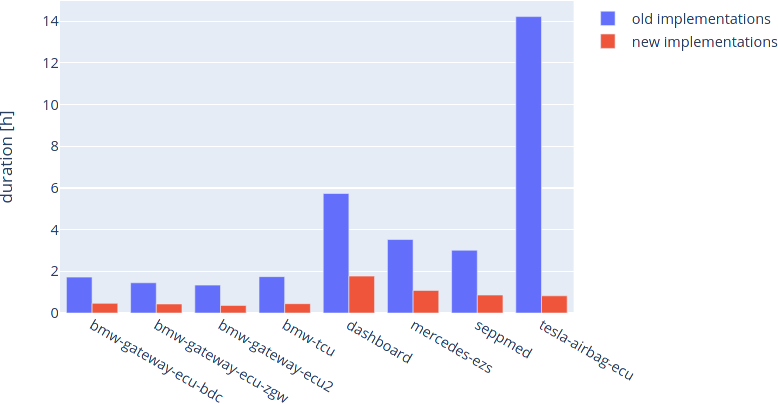
\includegraphics[width=1\textwidth]{durations-diff}
    \caption{Observed runtimes for a UDS scan with new implementations.}
    \label{fig:durations-diff}
\end{figure}

As \autoref{fig:durations-diff} illustrates, the speed-up is severe. Especially for the Tesla ECU the difference is huge.
This results from this ECU having a relatively high average response time (about 0.02 seconds) compared to the others (0.001 to 0.008 seconds).
